% !TeX program = luatex
% !TEX encoding = UTF-8


\documentclass{wg21}

\title{Pointer tagging for custom pointer types}
\docnumber{D4358R0}
\audience{LEWG}
\author{Corentin Jabot}{corentin.jabot@gmail.com}


\usepackage{color, colortbl}

% Macros used by [ptrtag] and by the de-tablified requirements which wg21.cls does not define yet.
\providecommand{\constantwhen}{\Fundesc{Constant When}}
\providecommand{\result}{\Fundesc{Result}}

% editing instructions, in the same purple wg21.cls uses for notes
\newcommand{\editinstr}[1]{\textcolor{noteclr}{#1}}

\begin{document}
\maketitle

\section{Abstract}

This paper propose to support pointer-like type in \tcode{pointer_tag_pair}.

\section{Motivation}

The recently added \tcode{pointer_tag_pair} require the pointer type to be an actual pointer, and does not support pointer-like user-defined types.
We propose a customization mechanism (\tcode{taggable\_pointer\_traits}) to support such types.

The motivational use cases are as follow:

\subsection{Opaque pointer types}

Opaque pointers, i.e classes that wraps a pointer in a type to block direct access to the pointer, or achieve some form of strong typing
are fairly common. And while their alignment bits are free, they are not accessible without the proposed \tcode{taggable\_pointer\_traits}.

Note that, it is not generally possible to use a smart / fancy /owning pointer with non-trivial constructor or destructor with this (or similar) interface.

\subsection{Nested pointer tagged pair}

An other use case, used a lot in LLVM, is to nest pointer_tag_pair.
For example, it is possible to define \tcode{pointer_tag_pair<pointer_tag_pair<int*, 1, unsigned>, 1, unsigned>}.
LLVM has complex structures and memory comes at a premium, so having to resort to that sort of optimization is fairly common.
This paper proposes a specialization of \tcode{taggable\_pointer\_traits} for \tcode{pointer_tag_pair} that make this possible.

\subsection{Function pointers}

While this goes a bit beyond what can be portably and conformingly achieved, \tcode{pointer_tag_pair} could be user-specialized
to allow storing a function pointer inside a \tcode{pointer_tag_pair}.

\subsection{Other uses for \tcode{taggable_pointer_traits}}

LLVM uses their equivalent of taggable_pointer_traits to store a discriminated union of pointer types in a single \tcode{void*}.
pointer-sized discriminated variant are a fairly common utility (Qt and Folluy have similar tools for example).
While we are not proposing such a type, \tcode{taggable_pointer_traits} can be reused for that use case (or anyother use case that want to query
alignment information of pointer like type).

\section{Design}

A trait, \tcode{taggable\_pointer\_traits} (for lack of a better name), offers the following interface

\begin{colorblock}

template <>
struct std::taggable_pointer_traits<T> {
    static constexpr unsigned bits_available = /*...*/;
    static constexpr void* to_void_pointer(T p) noexcept;
    static constexpr T from_void_pointer(void* v) noexcept;
};
\end{colorblock}

The standard provides a specialization for \tcode{pointer_int_pair} and \tcode{T*} (The primary tempolate is not defined).

The trait is queried by \tcode{pointer_int_pair}. in LLVM, the trait is a template parameter (like, e.g \tcode{char_traits} in string),
which offers an other layer of customization...which LLVM does not use, as far as I can tell.
The only use case I can imagine would be to customize the behavior for \tcode{void*} - which the standard considered to have an alignment
of \tcode{0} but it's sometimes to assume a greater alignment depending on use case and allocator.
However, a custom opaque pointer type over \tcode{void*}, or the use of \tcode{from_overaligned} would cover this use case.
Generally, any scenario where one would want to customize the behavior of a given pointer type can be  achieve by wrapping it in an opaque pointer type.

There are a few notable changes to the status quo:

\begin{itemize}
\item To support nested \tcode{pointer_tag_pair} work, we need to specify how the tag is stored rather than let it implementation defined.
  Ie the tag is stored in the high-most available least significant (alignment) bits.

\begin{figure}[htbp]
    \centering
    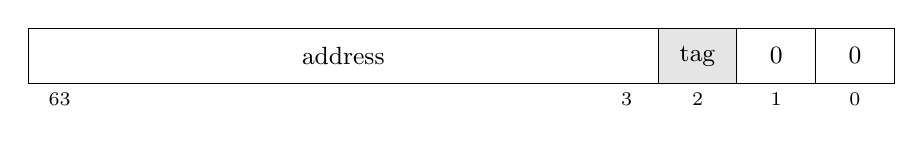
\begin{tikzpicture}[font=\small]
        \draw (0,0) rectangle (8,0.7);
        \draw[fill=black!10] (8,0) rectangle (9,0.7);
        \draw (9,0) rectangle (10,0.7);
        \draw (10,0) rectangle (11,0.7);
        \node at (4,0.35) {address};
        \node at (8.5,0.35) {tag};
        \node at (9.5,0.35) {0};
        \node at (10.5,0.35) {0};
        \node[below] at (0.4,0) {\scriptsize 63};
        \node[below] at (7.6,0) {\scriptsize 3};
        \node[below] at (8.5,0) {\scriptsize 2};
        \node[below] at (9.5,0) {\scriptsize 1};
        \node[below] at (10.5,0) {\scriptsize 0};
    \end{tikzpicture}
   % \caption{Tag placement in \tcode{pointer_tag_pair<T*, 1>} where \tcode{alignof(T)} is \tcode{8}.}
\end{figure}

\item \tcode{pointer_tag_pair::element_type} is removed, as it's unclear that all opaque pointer type could or would want to expose that information.

\item The \tcode{constexprness} of Hana's design remains, however user-defined specialization of the trait need not be \tcode{constexpr}.

\end{itemize}

\subsection{Open questions}

\begin{itemize}
\item The current design mandates the pointer-type to be default constructible. We could instead make \tcode{pointer_tag_pair} conditionally
default constructible.

\item I think we could provide a specialization of \tcode{taggable\_pointer\_traits} for \tcode{coroutine_handle}.

\end{itemize}


\subsection{What this is not}

Despite this paper extending \tcode{pointer_tag_pair} to non-pointer types, that utility still remainst very much build around
the idea of reusing pointer-alignment bits.
Some early feedback on this paper expressed a desire for more unused-bits optimizations including

\begin{itemize}
\item Tombsone values in \tcode{std::optional}.
\item Recycling of padding bits.
\item Owning pointer / tag pairs types (I'm not aware of anyone doing that?)
\item Pointer compressions
\item etc
\end{itemize}

This proposal is neither of these things. Each of this feature require different designs / controlling traits that the
interface of \tcode{pointer_tag_pair} or \tcode{taggable\_pointer\_traits} cannot accommodate.


\section{Implementation}

An implementation, based on Hana Dusíková's initial implementation of \paper{P3125R6} is available on
\href{https://compiler-explorer.com/z/or19xf7jM}{Compiler Exporer}. By virtue of it being a pure-library implementation,
it does not support using \tcode{pointer_tag_pair} as a constant expression.

\section{Wording}

\rSec1[memory.syn]{Header \tcode{<memory>} synopsis}

\editinstr{Modify \textbf{[memory.syn]} as indicated:}

\begin{codeblock}
namespace std {
  // [...]

  // [ptrtag], pointer tagging
  inline constexpr unsigned max_pointer_bits_available = @\seebelownc@;                 // freestanding
  constexpr unsigned pointer_bits_available(size_t alignment);                      // freestanding

  @\added{template<class Ptr> struct taggable\_pointer\_traits;}@ @\added{// freestanding}@

  @\removed{template<class T>}@
  @\removed{constexpr unsigned bits-available = pointer\_bits\_available(alignof(T));}@ @\removed{// \expos}@

  @\removed{template<class U> using element-of = pointer\_traits<U>::element\_type;}@@\removed{// \expos}@

  template<class Ptr, unsigned BitsRequested = @\removed{bits-available<element-of<Ptr>>}@@\added{taggable\_pointer\_traits<Ptr>::bits\_available}@,
           class TagT = unsigned>
    class pointer_tag_pair;                                                         // freestanding

  // [...]
}
\end{codeblock}

\rSec1[ptrtag]{Pointer tagging}

\editinstr{Insert a new subclause after \textbf{[ptrtag.bits]}:}

\begin{addedblock}

\rSec2[ptrtag.traits]{Taggable pointer traits}

\rSec3[ptrtag.traits.general]{General}

\pnum
\tcode{taggable_pointer_traits} provides an interface allowing the use of
a pointer-like type with \tcode{pointer_tag_pair}.

\indexlibraryglobal{taggable_pointer_traits}%
\begin{codeblock}
namespace std {
  template<class Ptr> struct taggable_pointer_traits;           // freestanding
}
\end{codeblock}

\pnum
A program may specialize \tcode{taggable_pointer_traits}
for a program-defined pointer type \iref{namespace.std}.

\pnum
\begin{note}
An operation of a \tcode{pointer_tag_pair} is usable in constant expressions
only if the traits operations are constant expressions.
\end{note}

\rSec3[ptrtag.traits.specializations]{\tcode{taggable_pointer_traits} specializations}

\pnum
Let \tcode{\exposid{COPY_CONST}(A, B)} be \tcode{const B}
if \tcode{A} is a const type, otherwise \tcode{B}.

\indexlibraryglobal{taggable_pointer_traits}%
\begin{codeblock}
namespace std {
  template<class T> struct taggable_pointer_traits<T*> {        // freestanding
    static constexpr unsigned bits_available = @\seebelow@;

    static constexpr @\exposid{COPY_CONST}@(T, void)* to_void_pointer(T* p) noexcept;
    static constexpr T* from_void_pointer(@\exposid{COPY_CONST}@(T, void)* v) noexcept;
  };
}
\end{codeblock}

\indexlibrarymember{bits_available}{taggable_pointer_traits}%
\begin{itemdecl}
static constexpr unsigned bits_available = @\seebelow@;
\end{itemdecl}

\begin{itemdescr}
\pnum
\tcode{bits_available} is \tcode{0} if \tcode{is_void_v<T>} is \tcode{true}, and
\tcode{pointer_bits_available(alignof(T))} otherwise.
\end{itemdescr}

\indexlibrarymember{to_void_pointer}{taggable_pointer_traits}%
\begin{itemdecl}
static constexpr @\exposid{COPY_CONST}@(T, void)* to_void_pointer(T* p) noexcept;
\end{itemdecl}

\begin{itemdescr}
\pnum
\returns
\tcode{p}.
\end{itemdescr}

\indexlibrarymember{from_void_pointer}{taggable_pointer_traits}%
\begin{itemdecl}
static constexpr T* from_void_pointer(@\exposid{COPY_CONST}@(T, void)* v) noexcept;
\end{itemdecl}

\begin{itemdescr}
\pnum
\returns
\tcode{static_cast<T*>(v)}.
\end{itemdescr}


\end{addedblock}

\rSec2[ptrtag.pair]{Class template \tcode{pointer_tag_pair}}

\rSec3[ptrtag.pair.general]{General}

\editinstr{Modify \textbf{[ptrtag.pair.general]} as indicated:}

\begin{codeblock}
namespace std {
  template<class U, class PtrT, unsigned BitsRequested, size_t Alignment = alignof(U)>
    concept @\exposconcept{tagging-compatible-pointee}@ =                        // \expos
      @\added{is\_pointer\_v<PtrT> \&\& is\_object\_v<U> \&\&}@
      @\libconcept{convertible_to}@<U*, PtrT> &&
      pointer_bits_available(Alignment) >= BitsRequested &&
      (is_void_v<@\removed{element-of}@@\added{remove\_pointer\_t}@<PtrT>> ||
       is_scalar_v<@\removed{element-of}@@\added{remove\_pointer\_t}@<PtrT>> ||
       is_union_v<@\removed{element-of}@@\added{remove\_pointer\_t}@<PtrT>> ||
       is_pointer_interconvertible_base_of_v<@\removed{element-of}@@\added{remove\_pointer\_t}@<PtrT>, U>);

  template<class TagT>
    constexpr unsigned @\exposidnc{tag-bit-width}@(TagT value) noexcept;      // \expos
  @\added{template<class TagT>}@
    @\added{constexpr uintptr\_t \exposidnc{tag-value}(TagT value) noexcept;}@              @\added{// \expos}@

  template<class Ptr, unsigned BitsRequested = @\removed{bits-available<element-of<Ptr>>}@@\added{taggable\_pointer\_traits<Ptr>::bits\_available}@,
           class TagT = unsigned>
  class pointer_tag_pair {                                      // freestanding
  public:
    using pointer_type        = Ptr;
    @\added{using traits\_type         = taggable\_pointer\_traits<Ptr>;}@
    @\removed{using element\_type        = pointer\_traits<Ptr>::element\_type;}@
    using tagged_pointer_type = @\seebelow@;
    using tag_type            = TagT;
    static constexpr unsigned bits_requested = BitsRequested;

    // [ptrtag.pair.cons], constructors
    constexpr pointer_tag_pair() noexcept;

    template<@\exposconcept{tagging-compatible-pointee}@<pointer_type, bits_requested> U>
      constexpr pointer_tag_pair(U* p, tag_type t);
    constexpr pointer_tag_pair(nullptr_t p, tag_type t);
    @\added{constexpr pointer\_tag\_pair(pointer\_type p, tag\_type t)}@
      @\added{requires (bits\_requested <= traits\_type::bits\_available);}@

    // [...]

    // [ptrtag.pair.comp], comparisons
    friend constexpr @\seebelow@ operator<=>(pointer_tag_pair lhs, pointer_tag_pair rhs)
      noexcept@\added{(see below)}@ requires @\added{three\_way\_comparable<pointer\_type> \&\&}@ @\libconcept{three_way_comparable}@<tag_type>;
    friend constexpr bool operator==(pointer_tag_pair, pointer_tag_pair)
      noexcept@\added{(see below)}@ requires @\added{equality\_comparable<pointer\_type> \&\&}@ @\libconcept{equality_comparable}@<tag_type>;
  };

  template<class Ptr>
    pointer_tag_pair(Ptr@\removed{*}@)
      -> pointer_tag_pair<Ptr@\removed{*}@>;
  template<class Ptr, class TagT>
    pointer_tag_pair(Ptr@\removed{*}@, TagT tag)
      -> pointer_tag_pair<Ptr@\removed{*}@, @\removed{bits-available<element-of<Ptr>>}@@\added{taggable\_pointer\_traits<Ptr>::bits\_available}@, TagT>;
}
\end{codeblock}

\pnum
\mandates
\begin{itemize}
\item \tcode{is_same_v<remove_cvref_t<Ptr>, Ptr>} is \tcode{true}.
\item \tcode{is_same_v<remove_cvref_t<TagT>, TagT>} is \tcode{true}.
\item \removed{\tcode{is_pointer_v<Ptr> \&\& !is_function_v<remove_pointer_t<Ptr>>} is \tcode{true}.}
\begin{addedblock}
\item \tcode{traits_type::bits_available <= max_pointer_bits_available}
is \tcode{true}.
\item \tcode{is_same_v<remove_const_t<remove_pointer_t<tagged_pointer_type>>, void>}
is \tcode{true}.
\item \tcode{is_same_v<decltype(traits_type::from_void_pointer(declval<tagged_pointer_type>())), Ptr>}
is \tcode{true}.
\item \tcode{is_default_constructible_v<Ptr>} is \tcode{true}.
\item \tcode{is_trivially_copyable_v<Ptr>} is \tcode{true}.
\item \tcode{sizeof(Ptr) == sizeof(uintptr_t) \&\& alignof(Ptr) == alignof(uintptr_t)} is \tcode{true}.
\item \tcode{noexcept(traits_type::to_void_pointer(declval<Ptr>()))} is \tcode{true}.
\item \tcode{noexcept(traits_type::from_void_pointer(declval<tagged_pointer_type>()))}
is \tcode{true}.
\end{addedblock}
\item \tcode{is_unsigned_v<UT>} is \tcode{true},
where \tcode{UT} is
\tcode{underlying_type_t<TagT>} if \tcode{TagT} is an enumeration type, and
\tcode{TagT} otherwise.
\item \removed{\tcode{sizeof(TagT) <= sizeof(void*)} is \tcode{true}.}
\item \tcode{BitsRequested <= max_pointer_bits_available} is \tcode{true}.
\end{itemize}

\editinstr{Add to \textbf{[ptrtag.pair.general]}:}

\begin{addedblock}

\pnum
Let \exposid{tag-shift} and \exposid{tag-mask} be as follow:
\begin{codeblock}
static constexpr unsigned @\exposid{tag-shift}@ =  // \expos
  traits_type::bits_available > bits_requested ? traits_type::bits_available - bits_requested : 0;
static constexpr uintptr_t @\exposid{tag-mask}@ =   // \expos
  ((uintptr_t(1) << bits_requested) - 1) << @\exposid{tag-shift}@;
\end{codeblock}

\pnum
\begin{note}
The tag occupies the most significant of the bits reported by
\tcode{traits_type::bits_available},
which leaves the \exposid{tag-shift} least significant bits of
the representation unused.
\end{note}

\indexlibraryglobal{\exposid{tag-value}}%
\begin{itemdecl}
template<class TagT> constexpr uintptr_t @\exposid{tag-value}@(TagT value) noexcept;
\end{itemdecl}

\begin{itemdescr}
\pnum
\returns
\tcode{static_cast<uintptr_t>(to_underlying(value))}
if \tcode{is_enum_v<TagT>} is \tcode{true},
otherwise \tcode{static_cast<uintptr_t>(value)}.
\end{itemdescr}

\end{addedblock}

\rSec3[ptrtag.pair.cons]{Constructors}

\editinstr{Modify \textbf{[ptrtag.pair.cons]} as indicated:}

\begin{itemdecl}
constexpr pointer_tag_pair() noexcept;
\end{itemdecl}

\begin{itemdescr}
\pnum
\ensures
\tcode{pointer()} is equal to \removed{\tcode{nullptr}}\added{\tcode{pointer_type()}} and
\tcode{tag()} is equal to \tcode{TagT()}.
\end{itemdescr}

\ednote{[...]}

\editinstr{Add to \textbf{[ptrtag.pair.cons]}:}

\begin{addedblock}

\indexlibraryglobal{pointer_tag_pair}%
\begin{itemdecl}
constexpr pointer_tag_pair(pointer_type p, tag_type t)
  requires (bits_requested <= traits_type::bits_available);
\end{itemdecl}

\begin{itemdescr}
\pnum
\constantwhen
Preconditions are met and
\tcode{traits_type::to_void_pointer(p)} is a constant expression.

\pnum
\expects
\begin{itemize}
\item \tcode{p} is not a pointer past the end of an object \iref{basic.compound}.
\item The \tcode{bits_requested} least significant bits of
\tcode{traits_type::to_void_pointer(p)} are zero.
\item \tcode{\exposid{tag-bit-width}(t) <= bits_requested} is \tcode{true}.
\end{itemize}

\pnum
\ensures
\tcode{pointer()} is equal to \tcode{p} and
\tcode{tag()} is equal to \tcode{t}.

\pnum
\throws
Nothing.
\end{itemdescr}

\end{addedblock}

\rSec3[ptrtag.pair.tagops]{Tagged pointer operations}

\editinstr{Modify \textbf{[ptrtag.pair.tagops]} as indicated:}

\indexlibraryglobal{tagged_pointer_type}%
\begin{itemdecl}
using tagged_pointer_type = @\seebelow@;
\end{itemdecl}

\begin{itemdescr}
\begin{removedblock}
\pnum
\tcode{tagged_pointer_type} denotes \cv{}~\tcode{void*},
for \cv{} such that pointer denotes \cv{}~\tcode{U*} for some type \tcode{U}.
\end{removedblock}
\begin{addedblock}
\pnum
\tcode{tagged_pointer_type} denotes the type of \tcode{traits_type::to_void_pointer(p)}
for a value \tcode{p} of type \tcode{pointer_type}.
\end{addedblock}
\end{itemdescr}

\indexlibraryglobal{tagged_pointer}%
\begin{itemdecl}
tagged_pointer_type tagged_pointer() const noexcept;
\end{itemdecl}

\begin{itemdescr}
\begin{removedblock}
\pnum
\returns
An unspecified value \tcode{tp} of \tcode{tagged_pointer_type} type
such that for any specialization \tcode{DP} of \tcode{pointer_tag_pair} and
alignment value \tcode{A} for which
\begin{itemize}
\item \tcode{pointer_bits_available(A) >= DP::bits_requested} is \tcode{true},
\item \tcode{is_sufficiently_aligned<A>(ptr)} is \tcode{true}, and
\item \tcode{\exposid{tag-bit-width}(tag) <= DP::bits_requested} is \tcode{true},
\end{itemize}
\tcode{DP::from_tagged(tp)} produces an object \tcode{dp} such that
\tcode{reinterpret_cast<pointer_type>(dp.pointer())} is equal to \tcode{ptr} and
\tcode{static_cast<TagT>(dp.tag())} is equal to \tcode{tag}.
\end{removedblock}

\begin{addedblock}
\pnum
\returns
A value \tcode{tp} of type \tcode{tagged_pointer_type} for which
the following expression is \tcode{true}:
\begin{codeblock}
bit_cast<uintptr_t>(tp) ==
  ((bit_cast<uintptr_t>(traits_type::to_void_pointer(pointer())) & ~@\exposid{tag-mask}@) |
   (@\exposid{tag-value}@(tag()) << @\exposid{tag-shift}@))
\end{codeblock}
\end{addedblock}

\pnum
\begin{note}
This function returns an invalid pointer value \iref{basic.compound}
with implementation-defined behavior \iref{ptrtag.bits}.
\end{note}
\end{itemdescr}

\indexlibraryglobal{from_tagged}%
\begin{itemdecl}
static pointer_tag_pair from_tagged(tagged_pointer_type p) noexcept;
\end{itemdecl}

\begin{itemdescr}
\begin{removedblock}
\pnum
\returns
An object \tcode{dp} of type \tcode{pointer_tag_type}, such that
\begin{itemize}
\item
\tcode{reinterpret_cast<pointer_type>(sp.pointer())} is equal to \tcode{dp.pointer()} and\\
\tcode{static_cast<TagT>(sp.tag())} is equal to \tcode{dp.tag()},
if \tcode{p} is equal to \tcode{sp.tagged_pointer()}
for some object \tcode{sp} of a type that is a specialization of \tcode{pointer_tag_type},
such that for some alignment value \tcode{A}
\begin{itemize}
\item \tcode{pointer_bits_available(A) >= bits_requested} is \tcode{true},
\item \tcode{is_sufficiently_aligned<A>(sp.pointer())} is \tcode{true}, and
\item \tcode{\exposid{tag-bit-width}(sp.tag()) <= bits_requested} is \tcode{true},
\end{itemize}
\item
otherwise, the values of \tcode{dp.pointer()} and \tcode{dp.tag()} are unspecified.
\end{itemize}
\end{removedblock}

\begin{addedblock}
\pnum
\returns
An object \tcode{ptp} of type \tcode{pointer_tag_pair} such that
\begin{itemize}
\item
\tcode{ptp.pointer()} is equal to
\tcode{traits_type::from_void_pointer(SP::traits_type::to_void_pointer(sp.pointer()))} and
\tcode{ptp.tag()} is equal to \tcode{static_cast<tag_type>(sp.tag())},
if \tcode{p} is equal to \tcode{sp.tagged_pointer()}
for some object \tcode{sp} of a type \tcode{SP}
that is a specialization of \tcode{pointer_tag_pair} for which
\begin{itemize}
\item \tcode{SP::\exposid{tag-shift}} is equal to \exposid{tag-shift}, and
\item \tcode{\exposid{tag-bit-width}(sp.tag()) <= bits_requested} is \tcode{true};
\end{itemize}
\item
otherwise, the values of \tcode{ptp.pointer()} and \tcode{ptp.tag()} are unspecified.
\end{itemize}
\end{addedblock}
\end{itemdescr}

\rSec3[ptrtag.pair.comp]{Comparisons}

\editinstr{Modify \textbf{[ptrtag.pair.comp]} as indicated:}

\indexlibrarymember{operator<=>}{pointer_tag_pair}%
\begin{itemdecl}
friend constexpr auto operator<=>(pointer_tag_pair lhs, pointer_tag_pair rhs)
  noexcept@\added{(see below)}@ requires @\added{three\_way\_comparable<pointer\_type> \&\&}@ @\libconcept{three_way_comparable}@<tag_type>;
\end{itemdecl}

\begin{itemdescr}
\pnum
\effects
Equivalent to:
\begin{codeblock}
return pair(lhs.pointer(), lhs.tag()) <=> pair(rhs.pointer(), rhs.tag());
\end{codeblock}

\begin{addedblock}
\pnum
\remarks
The exception specification is equivalent to
\tcode{noexcept(pair(lhs.pointer(), lhs.tag()) <=> pair(rhs.pointer(), rhs.tag()))}.
\end{addedblock}

\pnum
\recommended
Directly compare the internal bit representations
if the expression \tcode{lhs.tag() <=> rhs.tag()}
results in a call to a built-in operator \tcode{<=>}
comparing values of type \tcode{tag_type}\added{, and
the expression \tcode{lhs.pointer() <=> rhs.pointer()}
results in a call to a built-in operator \tcode{<=>}
comparing values of type \tcode{pointer_type}}.

\pnum
\begin{note}
The result of comparing unrelated pointers is unspecified.
\end{note}
\end{itemdescr}

\indexlibrarymember{operator==}{pointer_tag_pair}%
\begin{itemdecl}
friend constexpr bool operator==(pointer_tag_pair lhs, pointer_tag_pair rhs)
  noexcept@\added{(see below)}@ requires @\added{equality\_comparable<pointer\_type> \&\&}@ @\libconcept{equality_comparable}@<tag_type>;
\end{itemdecl}

\begin{itemdescr}
\pnum
\effects
Equivalent to:
\begin{codeblock}
return pair(lhs.pointer(), lhs.tag()) == pair(rhs.pointer(), rhs.tag());
\end{codeblock}

\begin{addedblock}
\pnum
\remarks
The exception specification is equivalent to
\tcode{noexcept(pair(lhs.pointer(), lhs.tag()) == pair(rhs.pointer(), rhs.tag()))}.
\end{addedblock}

\pnum
\recommended
Directly compare the internal bit representations
if the expression \tcode{lhs.tag() == rhs.tag()}
results in a call to a built-in operator \tcode{==}
comparing values of type \tcode{tag_type}\added{, and
the expression \tcode{lhs.pointer() == rhs.pointer()}
results in a call to a built-in operator \tcode{==}
comparing values of type \tcode{pointer_type}}.
\end{itemdescr}

\rSec3[ptrtag.pair.traits]{Taggable pointer traits for \tcode{pointer_tag_pair}}

\editinstr{Add a new subclause at the end of \textbf{[ptrtag.pair]}:}

\begin{addedblock}

\indexlibraryglobal{taggable_pointer_traits}%
\begin{codeblock}
namespace std {
  template<class Ptr, unsigned BitsRequested, class TagT>
  struct taggable_pointer_traits<                               // freestanding
    pointer_tag_pair<Ptr, BitsRequested, TagT>> {
    static constexpr unsigned bits_available = @\seebelow@;

    static pointer_tag_pair<Ptr, BitsRequested, TagT>::tagged_pointer_type
      to_void_pointer(pointer_tag_pair<Ptr, BitsRequested, TagT> p) noexcept;
    static pointer_tag_pair<Ptr, BitsRequested, TagT> from_void_pointer(
      pointer_tag_pair<Ptr, BitsRequested, TagT>::tagged_pointer_type v) noexcept;
  };
}
\end{codeblock}

\pnum
Let \tcode{PTP} denote \tcode{pointer_tag_pair<Ptr, BitsRequested, TagT>}.

\begin{itemdecl}
static constexpr unsigned bits_available = @\seebelow@;
\end{itemdecl}

\begin{itemdescr}
\pnum
\tcode{bits_available} is \tcode{PTP::\exposid{tag-shift}} \iref{ptrtag.pair.general}.
\end{itemdescr}

\begin{itemdecl}
static PTP::tagged_pointer_type to_void_pointer(PTP p) noexcept;
\end{itemdecl}

\begin{itemdescr}
\pnum
\returns
\tcode{p.tagged_pointer()}.
\end{itemdescr}

\begin{itemdecl}
static PTP from_void_pointer(PTP::tagged_pointer_type v) noexcept;
\end{itemdecl}

\begin{itemdescr}
\pnum
\returns
\tcode{PTP::from_tagged(v)}.
\end{itemdescr}


\end{addedblock}

\section{Feature test Macro}

\ednote{bump \tcode{__cpp_lib_pointer_tag_pair} to the date of adoption.}


\section{Acknowledgments}

Thanks to Hana Dusíková for her work on P3125R6, and for leaving the design open to the extension proposed here.

\bibliographystyle{plain}
\bibliography{wg21, extra}

\renewcommand{\section}[2]{}%

\begin{thebibliography}{9}

\bibitem[P3125R6]{P3125R6}
Hana Dusíková
\emph{constexpr pointer tagging}\newline
\url{https://wg21.link/P3125R6}

\bibitem[LLVMPointerIntPair]{LLVMPointerIntPair}
The LLVM Project
\emph{llvm::PointerIntPair Class Template Reference}\newline
\url{https://llvm.org/doxygen/classllvm_1_1PointerIntPair.html}

\bibitem[LLVM94324]{LLVM94324}
Nikolas Klauser
\emph{[libc++] Add \_\_pointer\_int\_pair}\newline
\url{https://github.com/llvm/llvm-project/pull/94324}

\bibitem[Tiny]{Tiny}
Jonathan Müller
\emph{tiny: \tcode{pointer_variant_impl} and \tcode{pointer_tiny_storage}}\newline
\url{https://github.com/foonathan/tiny}

\bibitem[QBiPointer]{QBiPointer}
The Qt Project
\emph{\tcode{QBiPointer}}\newline
\url{https://github.com/qt/qtdeclarative/blob/dev/src/qml/qml/ftw/qbipointer_p.h}

\bibitem[DiscriminatedPtr]{DiscriminatedPtr}
Meta
\emph{\tcode{folly::DiscriminatedPtr}}\newline
\url{https://github.com/facebook/folly/blob/main/folly/DiscriminatedPtr.h}

\end{thebibliography}

\end{document}
